\documentclass{beamer}

\mode<presentation>
{
  \usetheme{Frankfurt}
  \setbeamercovered{transparent}
  %\usecolortheme{whale}
}

\usepackage[english]{babel}
\usepackage[latin1]{inputenc}
\usepackage{times}
\usepackage[T1]{fontenc} 
% Or whatever. Note that the encoding and the font should match. If T1
% does not look nice, try deleting the line with the fontenc.
\usepackage{amsmath}
\usepackage{algorithmic}


\newcommand{\linespace}{\vskip 0.25cm}

\definecolor{MyForestGreen}{rgb}{0,0.7,0} 
\newcommand{\tableemph}[1]{{#1}}
\newcommand{\tablewin}[1]{\tableemph{#1}}
\newcommand{\tablemid}[1]{\tableemph{#1}}
\newcommand{\tablelose}[1]{\tableemph{#1}}

\definecolor{MyLightGray}{rgb}{0.6,0.6,0.6}
\newcommand{\tabletie}[1]{\color{MyLightGray} {#1}}

% The text in square brackets is the short version of your title and will be used in the
% header/footer depending on your theme.
\title[Intrusion Detection]{Intrusion Detection with \\ Genetic Algorithms and Fuzzy Logic}

% Sub-titles are optional - uncomment and edit the next line if you want one.
% \subtitle{Why does sub-tree crossover work?} 

% The text in square brackets is the short version of your name(s) and will be used in the
% header/footer depending on your theme.
\author[Ireland]{Emma Ireland}

% The text in square brackets is the short version of your institution and will be used in the
% header/footer depending on your theme.
\institute[U of Minn, Morris]
{
  Division of Science and Mathematics \\
  University of Minnesota, Morris \\
  Morris, Minnesota, USA
}

% The text in square brackets is the short version of the date if you need that.
\date[December 2013] % (optional)
{December 2013 \\ UMM CSci Senior Seminar Conference}

% Delete this, if you do not want the table of contents to pop up at
% the beginning of each subsection:
\AtBeginSection[]
{
  \begin{frame}<beamer>
    \frametitle{Outline}
    \tableofcontents[currentsection, hideothersubsections]
  \end{frame}
}

\begin{document}

\begin{frame}
  \titlepage
\end{frame}

% For a 20-25 minute senior seminar talk you probably want something like:
% - Two or three major sections (other than the summary).
% - At *most* three subsections per section.
% - Talk about 30s to 2min per frame. So there should probably be between
%   15 and 30 frames, all told.

\section*{Overview}

\subsection*{The Big Picture}

\begin{frame}
  \frametitle{The Big Picture}
  \begin{itemize}
  	\item Computer lab gets large numbers of login attempts that are attempts at intrusion.
	\begin{itemize}
		\item Trying to gain root access to the system.
		\item Delete files of other users and change user passwords.
	\end{itemize}
	\linespace
	\item With an intrusion detection system (IDS) -> classify those attempts.
	\item Intrusion detection systems provide one way of detecting attacks by monitoring network activities for malicious or abnormal behaviors and then producing reports, alerts, and actions.
	\item Training an IDS: use a fuzzy genetic algorithm.
  \end{itemize}
\end{frame}

\subsection*{Outline}

\begin{frame}
  \frametitle{Outline}
  \tableofcontents[hideallsubsections]
\end{frame}
%%%%%%%%%%%%%%%%%%%%%%%%%%%%%%%%%%%%%%%%%%%%%%%%%%%%%%%%%%%%%%%%%%%%%%%%%%%%%%%%%
%%%%%%%%%%%%%%%%%%%%%%%%%%%%%%%%%%%%%%%%%%%%%%%%%%%%%%%%%%%%%%%%%%%%%%%%%%%%%%%%%
%%%%%%%%%%%%%%%%%%%%%%%%%%%%%%%%%%%%%%%%%%%%%%%%%%%%%%%%%%%%%%%%%%%%%%%%%%%%%%%%%
%%%%%%%%%%%%%%%%%%%%%%%%%%%%%%%%%%%%%%%%%%%%%%%%%%%%%%%%%%%%%%%%%%%%%%%%%%%%%%%%%
\section[Intrusion Detection]{Intrusion Detection}
\subsection{Types of Networking Attacks}
\begin{frame}
  \frametitle{Types of Networking Attacks}
  \begin{itemize}
  	\item Denial of Service (DoS): 
  	
  	makes machine inaccessible to user by making it too busy to serve legitimate requests.
  	
  	\begin{itemize}
  		\item  Systems lock out user from account after certain number of failed login attempts. Attacker would be able to use this to prevent users from logging in, by failing to log in enough times to lock the account.
  	\end{itemize}

  	\linespace
  	\linespace
  	
  	\item Probe: 
  	
  	examines machine in order to collect information about weaknesses that in the future could be used to compromise the system.
  	
  	\begin{itemize}
  		\item Attacker could be trying to determine what version of a software is being run on that machine, and if that version has a known issue then that allows them to attempt to attack that.
  	\end{itemize}
  \end{itemize}
\end{frame}


\subsection{Detection Methodologies}
\begin{frame}
  \frametitle{Detection Methodologies}
  \begin{itemize}
  	\item Signature-based detection: compares well-known patterns of attacks
that are already known to the IDS against captured events in order to identify a possible attack.
	\begin{itemize}
		\item Simple and effective way to detect known attacks, 
		
		ineffective against new kinds of unknown attacks.
	\end{itemize}

\linespace
\linespace

  	\item Anomaly-based detection: looks for patterns of activity that are rare and uncommon.
	\begin{itemize}
		\item Harder to do than signature-based detection, 
		
		can be an effective way to detect new, unknown attacks.
	\end{itemize}
  \end{itemize}
\end{frame}


\subsection{Data Sets - KDD99 and RLD09}
\begin{frame}
  \frametitle{KDD99}
	\begin{itemize}
		\item Generated by simulating a military network environment in 1999.
		\item Has long been a standard data set for intrusion detection.
		
\linespace		
		
		\item Data was processed into 5 million \emph{records}.
			\begin{itemize}
				\item A record is a sequence of TCP packets, between which data flows to and from a source IP address to a target IP address.
			\end{itemize}
		\item Each record is classified as either normal or attack activity.
	\end{itemize}
\end{frame}


\begin{frame}
  \frametitle{Features of KDD99}
	\begin{itemize}
		\item KDD99 uses 41 \emph{features}, which are properties of a record that are used to describe the activity and help to distinguish normal connections from attacks.
		
		\linespace
		\linespace
		
		\item duration: length of the record in seconds.
		\item num\_failed\_logins: number of failed login attempts.
		\item root\_shell: returns 1 if root shell is obtained, else returns 0.
	\end{itemize}
\end{frame}



\begin{frame}
  \frametitle{RLD09}
	\begin{itemize}
		\item RLD09 was created because KDD99 is 14 years old, 
		
		newer attack types are not in KDD99 because of its age.
		\item Data was captured from a university in Bangkok, Thailand.
		\item As well as normal network activity, has 17 different types of attacks (divided into denial of service and probe attacks).
	\end{itemize}
\end{frame}



\begin{frame}
  \frametitle{Rules}
	\begin{itemize}
		\item A commonly used approach for detecting intrusions is to use rules.
		\item If-Then format: If (\emph{condition}) then (\emph{consequence}).
		\begin{itemize}
			\item The condition is composed of one or more features, and the consequence says if it is an intrusion or not.
			\item If \emph{duration = 4} then \emph{intrusion}.
		\end{itemize}				
	\end{itemize}
\end{frame}



\begin{frame}
  \frametitle{Training and Testing Sets}
	\begin{itemize}
		\item The authors divided the data set into two subsets, a \emph{training set} and a \emph{test set}.
        \item The given algorithm is then trained on the training set to look for patterns.
        \item These patterns are then verified using the test set.
	\end{itemize}
\end{frame}



\subsection{Determining the Accuracy of an Algorithm}
\begin{frame}
  \frametitle{Determining the Accuracy of an Algorithm}
%\centering{Predicted}
\begin{table}
%Actual
Predicted
\begin{tabular}{l|ll}
Actual   & Not Attack & Attack \\ \hline
Not Attack & True Negative (TN) & False Positive (FP) \\
Attack & False Negative (FN) & True Positive (TP)  \\
\end{tabular}
\end{table}
\linespace
\linespace
\begin{center}
Detection rate (DR): percentage of normal and attack activity correctly classified from the total number of data records.
\end{center}
\end{frame}
%%%%%%%%%%%%%%%%%%%%%%%%%%%%%%%%%%%%%%%%%%%%%%%%%%%%%%%%%%%%%%%%%%%%%%%%%%%%%%%%%
%%%%%%%%%%%%%%%%%%%%%%%%%%%%%%%%%%%%%%%%%%%%%%%%%%%%%%%%%%%%%%%%%%%%%%%%%%%%%%%%%
\section[Fuzzy Algorithm]{Fuzzy Algorithm}
\subsection{Fuzzy Logic}
\begin{frame}
	\frametitle{Fuzzy Logic}
	\begin{itemize}
		\item Fuzzy logic is used in intrusion detection systems to find the degree of certainty of a record being an attack.
		\item Fuzzy logic rules are similar to the rules described before, except that
consequence is a certainty factor. 
		\begin{itemize}
			\item If (\emph{duration} = 6) then (\emph{the degree of certainty of the record being an attack is 0.5}).
		\end{itemize}
	\end{itemize}
\end{frame}

\subsection{Finding the Degree of Certainty}
\begin{frame}
  \frametitle{Finding the Degree of Certainty of a Record Being an Attack}
	Suppose that the feature is duration, and it is 6 seconds. Then data=6.
  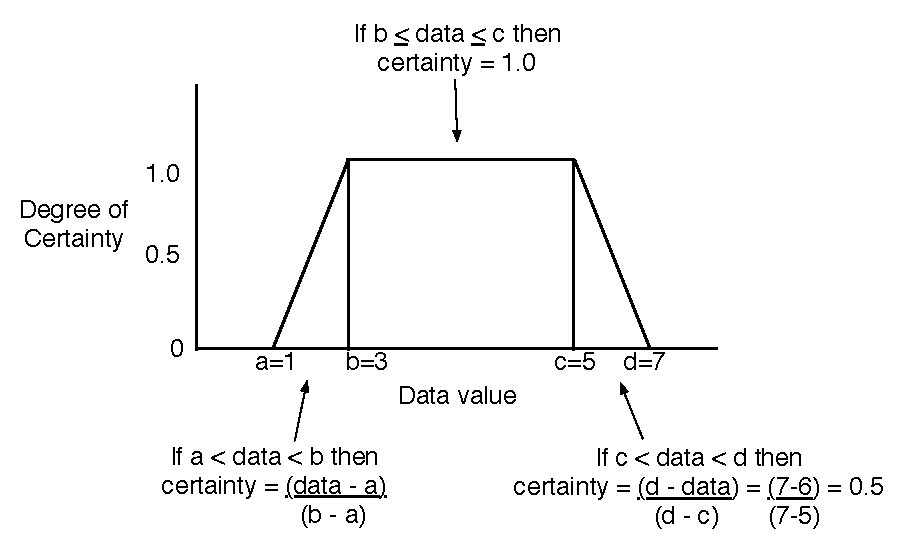
\includegraphics[width=0.95\textwidth]{../trapFigExample.pdf}
\end{frame}


\subsection{Encoding of Features and Rules}
\begin{frame}
	\frametitle{Encoding of Features and Rules}
	\begin{itemize}
	\item The four parameters are encoded into blocks. Each block is a feature with values between 0 and 7.
	\item A rule has one block for each of 12 features followed at the end by a marker indicating the type of attack.
	\end{itemize}

\begin{figure}
\begin{small}
\begin{tabular}{|cccc|c|cccc|c|} \hline
010 & 011 & 100 & 101   & ... & 010 & 011 & 101 & 111   & Attack\\
a=2 & b=3 & c=4 & d=5   & ... & a=2 & b=3 & c=5 & d=7   &\\ 
    &     & Block 1&    &        &     & Block 12& &       & Type\\
\hline\end{tabular}
\caption{Based on [Jongsuebsuk \emph{et al.}, 2013]}
\end{small}
\end{figure}

	\begin{itemize}
		\item The degree of certainty is computed for each of the 12 blocks, and if the sum of those is greater than a threshold, then it will be declared as an attack.
	\end{itemize}

\end{frame}
%%%%%%%%%%%%%%%%%%%%%%%%%%%%%%%%%%%%%%%%%%%%%%%%%%%%%%%%%%%%%%%%%%%%%%%%%%%%%%%%%
%%%%%%%%%%%%%%%%%%%%%%%%%%%%%%%%%%%%%%%%%%%%%%%%%%%%%%%%%%%%%%%%%%%%%%%%%%%%%%%%%
\section[Genetic Algorithms]{Genetic Algorithms}
\subsection{GA Overview}
\begin{frame}
  \frametitle{Genetic Algorithms}
	\begin{itemize}
		\item GAs: search technique used to find solutions to problems.
        \item Possible solutions to problems can be represented in a variety of problem dependent ways, such as bit strings.
        
        \begin{itemize}
        	\item IDS rules can be represented as bit strings.
        \end{itemize}
        
        \linespace
        \item First, randomly generated population of potential solutions is created. Mutation, crossover, selection are applied to each generation until acceptable solution is found or some time limit is exceeded.
	\end{itemize}
\end{frame}


\subsection{Mutation and Crossover}
\begin{frame}
  \frametitle{Mutation and Crossover}
	\begin{itemize}
        \item Mutation: random bits in an individual, or possible solution, are randomly changed.
        \begin{itemize}
        	\item Takes bits of rule and changes them to form slightly different rule.
        	
        	\begin{figure}
			\begin{tabular}{|cccc|} \hline
			010 & 011 & 100 & \textbf{101}\\
			a=2 & b=3 & c=4 & \textbf{d=5}\\
			\hline\end{tabular}
			$\rightarrow$
			\quad
			\begin{tabular}{|cccc|} \hline
			010 & 011 & 100 & \textbf{111}\\
			a=2 & b=3 & c=4 & \textbf{d=7}\\
			\hline\end{tabular}			
			\end{figure}
        \end{itemize}
        
        \linespace
        \linespace
        \linespace
        
        \item Crossover: two individuals swap sequences of bits to form two new individuals.
        \begin{itemize}
        	\item Take 2 rules and creates new rules by swapping bits of old rules.
        	
        	\begin{figure}
			\begin{tabular}{|cccc|} \hline
			001 & 011 & 101 & 111\\
			a=1 & b=3 & c=5 & d=7\\
			\hline\end{tabular}
			\quad
			\begin{tabular}{|cccc|} \hline
			010 & 100 & 110 & 111\\
			a=2 & b=4 & c=6 & d=7\\
			\hline\end{tabular}			
			\end{figure}
        \end{itemize}
	\end{itemize}
\end{frame}


\subsection{Selection and Fitness}
\begin{frame}
  \frametitle{Selection and Fitness}
	\begin{itemize}
        \item Selection: individuals that have better fitness are chosen to be parents.
        \item The fitness of an individual is specified by the fitness function, which determines the quality of a particular individual.
        
        \linespace
        \linespace
        
       	\item In an IDS: fitness measures how well a rule classifies records as either attacks or normal activity. Selection combined with fitness function directs search towards effective solution.
	\end{itemize}
\end{frame}


\begin{frame}
	\frametitle{Fitness function}
	The fitness function in the algorithm is:
	\begin{equation*}
	\frac{\alpha}{A} - \frac{\beta}{B}
	\end{equation*}

	$\alpha$: \# of attack records correctly identified as attack.

	$A$: \# of attack records.

	$\beta$: \# of normal records incorrectly classified as attack.
	
	$B$: \# of normal records.
\end{frame}
%%%%%%%%%%%%%%%%%%%%%%%%%%%%%%%%%%%%%%%%%%%%%%%%%%%%%%%%%%%%%%%%%%%%%%%%%%%%%%%%%
%%%%%%%%%%%%%%%%%%%%%%%%%%%%%%%%%%%%%%%%%%%%%%%%%%%%%%%%%%%%%%%%%%%%%%%%%%%%%%%%%
%%%%%%%%%%%%%%%%%%%%%%%%%%%%%%%%%%%%%%%%%%%%%%%%%%%%%%%%%%%%%%%%%%%%%%%%%%%%%%%%%
%%%%%%%%%%%%%%%%%%%%%%%%%%%%%%%%%%%%%%%%%%%%%%%%%%%%%%%%%%%%%%%%%%%%%%%%%%%%%%%%%
\section[Experiments and Results]{Experiments and Results}
\subsection{Two Experiments using Only RLD09}
\begin{frame}
	\frametitle{Experiments Using Only RLD09}
	Experiment 1
	\begin{itemize}
		\item Fuzzy GA was used to create DoS and probe detection rules. 
		
		Both rules were then used together in testing process to identify attacks from testing data set.
		
		\linespace
		\linespace
		
		\item Training set: 10,000 records.
		
		Test set: 26,500 records.

		\linespace
		\linespace

		\item If the record is either a DoS rule or a Probe rule, it is classified as an attack; else it is normal.
\end{itemize}
\end{frame}


\begin{frame}
	\frametitle{Experiments Using Only RLD09}
	Experiment 1 Results
\begin{table}
\begin{small}
\begin{tabular}{lllllll}
 & Attack & Normal & Total & FP(\%) & FN(\%) & DR(\%)\\
DoS Training & 1499 & 8501 & 10000 & 1.46 & 47.50 & 91.64\\
Probe Training & 2496 & 7504 & 10000 & 1.83 & 15.38 & 94.79\\
Testing & 10500 & 16000 & 26500 & 1.13 & 4.10 & 97.92\\
\end{tabular}
\end{small}
\end{table}
\end{frame}


\begin{frame}
	\frametitle{Experiments Using Only RLD09}
Experiment 2
	\begin{itemize}
		\item Attacks pulled out of training set and kept for unknown data testing, to test that fuzzy GA could detect unknown attacks.
		\item Used fuzzy GA and a decision tree algorithm, which is another common algorithm for classification problems.
		\item 7 tests were run. 
		
		For each test case there were 13 attack types plus normal activity that were in the training data set. 
		
		3 attack types were used for the unknown testing data set.
	\end{itemize}
\end{frame}


\begin{frame}
	\frametitle{Experiments Using Only RLD09}
	Experiment 2 Results (7 tests were run in total, 5 are shown here.)
	
\begin{table}
\begin{footnotesize}
\begin{tabular}{llll}
Test & Unknown & Decision & Fuzzy\\
Case & Attacks & Tree DR (\%) & Genetic DR (\%)\\ \hline

1 & Adv Port Scan (Probe) & Avg = & Avg =\\
  & Ack Scan (Probe)                 & 98.33 & 100\\
  & Xmas Tree (Probe)                 &                 &\\ \hline

2 & UDP Flood (DoS) & Avg = & Avg =\\
  & Host Scan (Probe) & 46.65 & 99.80\\
  & UDP Scan (Probe) & &\\ \hline

3 & Jping (DoS) & Avg = & Avg =\\
  & Syn Scan (Probe) & 99.70 & 98.75\\
  & Fin Scan (Probe) & &\\ \hline

4 & UDP Flood (DoS) & Avg = & Avg =\\
  & RCP Scan (Probe) & 70.35 & 98.15\\
  & Fin Scan (Probe) & &\\ \hline

5 & Http Flood (DoS) & Avg = & Avg =\\
  & RCP Scan (Probe) & 99.94 & 97.50\\
  & Fin Scan (Probe) & &\\
\hline\end{tabular}
\end{footnotesize}
\end{table}
\end{frame}



\subsection{Three Experiments using Both RLD09 and KDD99}
\begin{frame}
	\frametitle{Experiments Using Both RLD09 and KDD99}
Three experiments used both RLD09 and KDD99.

\linespace
\linespace

Experiment 1 - Used fuzzy GA to classify normal activity and attacks from KDD99 and RLD09.
	
\begin{table}
\begin{tabular}{cccccc}
Data set & Attack & Normal & FP (\%) & FN (\%) & DR (\%)\\ \hline
KDD99 & 160,117 & 39,337 & 0.13 & 1.55 & 98.72\\
RLD09 & 10,500 & 16,000 & 1.14 & 3.39 & 97.97\\
\end{tabular}
\end{table}
\end{frame}


\begin{frame}
	\frametitle{Experiments Using Both RLD09 and KDD99}
Experiment 2
	\begin{itemize}
		\item Used the fuzzy GA to classify types of attacks in KDD99.
		\item 10 tests were run in total, 5 are shown here.
	\end{itemize}
\begin{table}
\begin{tabular}{cccccc}
Test & Attack & Type & FP (\%) & FN (\%) & DR (\%)\\ \hline
1 & Back & DoS & 85.33 & 0.00 & 16.56\\
2 & PoD & DoS & 84.66 & 0.00 & 15.58\\
3 & Smurf & DoS & 0.76 & 0.10 & 99.73\\
4 & Portsweep & Probe & 6.40 & 0.00 & 93.66\\
5 & Satan & Probe & 0.74 & 3.75 & 99.22\\
\end{tabular}
\end{table}

\begin{itemize}
	\item 8 test cases had DR greater than 93\%. Only 2 cases had low DR, (cases 1 and 2).
\end{itemize}

\end{frame}


\begin{frame}
	\frametitle{Experiments Using Both RLD09 and KDD99}
Experiment 3
	\begin{itemize}
		\item Used the fuzzy GA to classify types of attacks in RLD09.
		\item 17 tests were run in total, 6 are shown here.
	\end{itemize}
\begin{table}
\begin{tabular}{cccccc}
Test & Attack & Type & FP (\%) & FN (\%) & DR (\%)\\ \hline
1 & HTTP Flood & DoS & 0.36 & 3.5 & 99.46\\
2 & Smurf & DoS & 0.02 & 0 & 99.98\\
3 & UDP Flood & DoS & 11.06 & 0 & 89.59\\
4 & Fin Scan & Probe & 2.58 & 0 & 97.50\\
5 & IP Scan & Probe & 13.01 & 16.4 & 86.89\\
6 & Syn Scan & Probe & 0.65 & 4.2 & 99.24\\
\end{tabular}
\end{table}

\begin{itemize}
	\item 15 cases had DR greater than 97\%. 2 cases had low DR, (cases 3 and 5).
\end{itemize}

\end{frame}
%%%%%%%%%%%%%%%%%%%%%%%%%%%%%%%%%%%%%%%%%%%%%%%%%%%%%%%%%%%%%%%%%%%%%%%%%%%%%%%%%
%%%%%%%%%%%%%%%%%%%%%%%%%%%%%%%%%%%%%%%%%%%%%%%%%%%%%%%%%%%%%%%%%%%%%%%%%%%%%%%%%
%%%%%%%%%%%%%%%%%%%%%%%%%%%%%%%%%%%%%%%%%%%%%%%%%%%%%%%%%%%%%%%%%%%%%%%%%%%%%%%%%
%%%%%%%%%%%%%%%%%%%%%%%%%%%%%%%%%%%%%%%%%%%%%%%%%%%%%%%%%%%%%%%%%%%%%%%%%%%%%%%%%
\section[Conclusions]{Conclusions}

\begin{frame}
\frametitle{Conclusions}
	\begin{itemize}
		\item The fuzzy genetic algorithm had a higher detection rate than a decision tree algorithm in most cases.
		\item Fuzzy genetic algorithms are good at detecting unknown attacks.
		\item The use of fuzzy genetic algorithms in intrusion detection is an effective way of detecting attacks.
	\end{itemize}
\end{frame}


\begin{frame}
	\frametitle{Thanks!}
	
	Thank you for your time and attention!
		
	\linespace
	\linespace
	
	\begin{center}
	{\Large Questions?}
	\end{center}
\end{frame}


\begin{frame}
	\frametitle{Probe Attacks}
	\begin{itemize}
		\item Advance Port Scan
		\item Ack Scan
		\item Xmas Tree
		\item Host Scan
		\item UDP Scan
		\item Syn Scan
		\item Fin Scan
		\item RCP Scan
		\item Portsweep
		\item Satan
		\item IP Scan
	\end{itemize}
\end{frame}


\begin{frame}
	\frametitle{DoS Attacks}
	\begin{itemize}
		\item UDP Flood
		\item Jping
		\item HTTP Flood
		\item Back
		\item PoD
		\item Smurf
	\end{itemize}
\end{frame}

\section*{References}

\begin{frame} 
	\frametitle{References} 
	
	\begin{thebibliography}{lskdjf}
	
	\begin{small}
	\bibitem{6496342}
Jongsuebsuk, P. and Wattanapongsakorn, N. and Charnsripinyo, C.
\newblock Network intrusion detection with Fuzzy Genetic Algorithm for unknown attacks.
\newblock In \emph{2013 International Conference on Information Networking (ICOIN)}, pages 1-5, 2013.
	
	
	\bibitem{6559603}
Jongsuebsuk, P. and Wattanapongsakorn, N. and Charnsripinyo, C.
\newblock Real-time intrusion detection with fuzzy genetic algorithm.
\newblock In \emph{2013 10th International Conference on Electrical Engineering/Electronics, Computer, Telecommunications and Information Technology (ECTI-CON)}, pages 1-6, 2013.
	\end{small}
	
  	\end{thebibliography}
  	
  	\linespace
  	
  	\begin{center}
  	\begin{small}
  	See my Senior Seminar paper for additional references.
  	\end{small}
  	\end{center}
	
\end{frame} 

\end{document}


